\documentclass[]{article}
\usepackage{lmodern}
\usepackage{amssymb,amsmath}
\usepackage{ifxetex,ifluatex}
\usepackage{fixltx2e} % provides \textsubscript
\ifnum 0\ifxetex 1\fi\ifluatex 1\fi=0 % if pdftex
  \usepackage[T1]{fontenc}
  \usepackage[utf8]{inputenc}
\else % if luatex or xelatex
  \ifxetex
    \usepackage{mathspec}
  \else
    \usepackage{fontspec}
  \fi
  \defaultfontfeatures{Ligatures=TeX,Scale=MatchLowercase}
  \newcommand{\euro}{€}
\fi
% use upquote if available, for straight quotes in verbatim environments
\IfFileExists{upquote.sty}{\usepackage{upquote}}{}
% use microtype if available
\IfFileExists{microtype.sty}{%
\usepackage{microtype}
\UseMicrotypeSet[protrusion]{basicmath} % disable protrusion for tt fonts
}{}


\usepackage{longtable,booktabs}
\usepackage{graphicx,grffile}
\makeatletter
\def\maxwidth{\ifdim\Gin@nat@width>\linewidth\linewidth\else\Gin@nat@width\fi}
\def\maxheight{\ifdim\Gin@nat@height>\textheight\textheight\else\Gin@nat@height\fi}
\makeatother
% Scale images if necessary, so that they will not overflow the page
% margins by default, and it is still possible to overwrite the defaults
% using explicit options in \includegraphics[width, height, ...]{}
\setkeys{Gin}{width=\maxwidth,height=\maxheight,keepaspectratio}
\setlength{\parindent}{0pt}
\setlength{\parskip}{6pt plus 2pt minus 1pt}
\setlength{\emergencystretch}{3em}  % prevent overfull lines
\providecommand{\tightlist}{%
  \setlength{\itemsep}{0pt}\setlength{\parskip}{0pt}}
\setcounter{secnumdepth}{5}

%%% Use protect on footnotes to avoid problems with footnotes in titles
\let\rmarkdownfootnote\footnote%
\def\footnote{\protect\rmarkdownfootnote}

%%% Change title format to be more compact
\usepackage{titling}

\RequirePackage[]{/Library/Frameworks/R.framework/Versions/3.4/Resources/library/BiocStyle/resources/tex/Bioconductor2}

% Create subtitle command for use in maketitle
\newcommand{\subtitle}[1]{
  \posttitle{
    \begin{center}\large#1\end{center}
    }
}

\setlength{\droptitle}{-2em}
\bioctitle[]{powerTCR}
  \pretitle{\vspace{\droptitle}\centering\huge}
  \posttitle{\par}
\author{Hillary Koch}
  \preauthor{\centering\large\emph}
  \postauthor{\par}
  \predate{\centering\large\emph}
  \postdate{\par}
  \date{2 February 2018}


% Redefines (sub)paragraphs to behave more like sections
\ifx\paragraph\undefined\else
\let\oldparagraph\paragraph
\renewcommand{\paragraph}[1]{\oldparagraph{#1}\mbox{}}
\fi
\ifx\subparagraph\undefined\else
\let\oldsubparagraph\subparagraph
\renewcommand{\subparagraph}[1]{\oldsubparagraph{#1}\mbox{}}
\fi

% code highlighting
\definecolor{fgcolor}{rgb}{0.251, 0.251, 0.251}
\newcommand{\hlnum}[1]{\textcolor[rgb]{0.816,0.125,0.439}{#1}}%
\newcommand{\hlstr}[1]{\textcolor[rgb]{0.251,0.627,0.251}{#1}}%
\newcommand{\hlcom}[1]{\textcolor[rgb]{0.502,0.502,0.502}{\textit{#1}}}%
\newcommand{\hlopt}[1]{\textcolor[rgb]{0,0,0}{#1}}%
\newcommand{\hlstd}[1]{\textcolor[rgb]{0.251,0.251,0.251}{#1}}%
\newcommand{\hlkwa}[1]{\textcolor[rgb]{0.125,0.125,0.941}{#1}}%
\newcommand{\hlkwb}[1]{\textcolor[rgb]{0,0,0}{#1}}%
\newcommand{\hlkwc}[1]{\textcolor[rgb]{0.251,0.251,0.251}{#1}}%
\newcommand{\hlkwd}[1]{\textcolor[rgb]{0.878,0.439,0.125}{#1}}%
\let\hlipl\hlkwb
%
\usepackage{fancyvrb}
\newcommand{\VerbBar}{|}
\newcommand{\VERB}{\Verb[commandchars=\\\{\}]}
\DefineVerbatimEnvironment{Highlighting}{Verbatim}{commandchars=\\\{\}}
%
\newenvironment{Shaded}{\begin{myshaded}}{\end{myshaded}}
% set background for result chunks
\let\oldverbatim\verbatim
\renewenvironment{verbatim}{\color{codecolor}\begin{myshaded}\begin{oldverbatim}}{\end{oldverbatim}\end{myshaded}}
%
\newcommand{\KeywordTok}[1]{\hlkwd{#1}}
\newcommand{\DataTypeTok}[1]{\hlkwc{#1}}
\newcommand{\DecValTok}[1]{\hlnum{#1}}
\newcommand{\BaseNTok}[1]{\hlnum{#1}}
\newcommand{\FloatTok}[1]{\hlnum{#1}}
\newcommand{\ConstantTok}[1]{\hlnum{#1}}
\newcommand{\CharTok}[1]{\hlstr{#1}}
\newcommand{\SpecialCharTok}[1]{\hlstr{#1}}
\newcommand{\StringTok}[1]{\hlstr{#1}}
\newcommand{\VerbatimStringTok}[1]{\hlstr{#1}}
\newcommand{\SpecialStringTok}[1]{\hlstr{#1}}
\newcommand{\ImportTok}[1]{{#1}}
\newcommand{\CommentTok}[1]{\hlcom{#1}}
\newcommand{\DocumentationTok}[1]{\hlcom{#1}}
\newcommand{\AnnotationTok}[1]{\hlcom{#1}}
\newcommand{\CommentVarTok}[1]{\hlcom{#1}}
\newcommand{\OtherTok}[1]{{#1}}
\newcommand{\FunctionTok}[1]{\hlstd{#1}}
\newcommand{\VariableTok}[1]{\hlstd{#1}}
\newcommand{\ControlFlowTok}[1]{\hlkwd{#1}}
\newcommand{\OperatorTok}[1]{\hlopt{#1}}
\newcommand{\BuiltInTok}[1]{{#1}}
\newcommand{\ExtensionTok}[1]{{#1}}
\newcommand{\PreprocessorTok}[1]{\textit{#1}}
\newcommand{\AttributeTok}[1]{{#1}}
\newcommand{\RegionMarkerTok}[1]{{#1}}
\newcommand{\InformationTok}[1]{\textcolor{messagecolor}{#1}}
\newcommand{\WarningTok}[1]{\textcolor{warningcolor}{#1}}
\newcommand{\AlertTok}[1]{\textcolor{errorcolor}{#1}}
\newcommand{\ErrorTok}[1]{\textcolor{errorcolor}{#1}}
\newcommand{\NormalTok}[1]{\hlstd{#1}}
%
\AtBeginDocument{\bibliographystyle{/Library/Frameworks/R.framework/Versions/3.4/Resources/library/BiocStyle/resources/tex/unsrturl}}

\usepackage{amsthm}
\newtheorem{theorem}{Theorem}[section]
\newtheorem{lemma}{Lemma}[section]
\theoremstyle{definition}
\newtheorem{definition}{Definition}[section]
\newtheorem{corollary}{Corollary}[section]
\newtheorem{proposition}{Proposition}[section]
\theoremstyle{definition}
\newtheorem{example}{Example}[section]
\theoremstyle{definition}
\newtheorem{exercise}{Exercise}[section]
\theoremstyle{remark}
\newtheorem*{remark}{Remark}
\newtheorem*{solution}{Solution}
\begin{document}
\maketitle
\begin{abstract}
This vignette walks through the functionality of the powerTCR package
for analyzing the T cell receptor repertoire. The package's main goals
are to fit models to the clone size distribution of the TCR repertoire,
and to perform model-based comparative analysis of samples, following
the work of \textbf{my paper}. For user simplicity, powerTCR can handle
data in the formats MiTCR, MiTCR with UMIs, MiGEC, VDJtools, ImmunoSEQ
(both old and new), MiXCR, and IMSEQ. If not using one of these formats,
powerTCR only requires that the user be able to turn a sample TCR
repertoire into a vector of clone sizes.
\end{abstract}

\packageVersion{powerTCR 0.1.0}

{
\setcounter{tocdepth}{2}
\tableofcontents
\newpage
}
\section{Introduction}\label{introduction}

The powerTCR package allows users to implement the model-based methods
discussed in \textbf{my paper}. Specifically, the clone size
distribution of the T cell receptor (TCR) repertoire exhibits imperfect
power law behavior; powerTCR supports a model that keeps this fact in
mind. Additionally, powerTCR contains tools to fit another power law
model for the TCR repertoire detailed in Desponds et al. (2016). Given a
collection of sampled TCR repertoires, powerTCR equips the user with
tools for comparative analysis of the samples, using one of two
model-based approaches. This leads to hierarchical clustering of the
samples to determine their relatedness based on the clone size
distribution alone.

\subsection{Summary of features}\label{summary-of-features}

\begin{itemize}
\tightlist
\item
  Read in and parse TCR sequencing files stored in various formats into
  the necessary format for powerTCR
\item
  Fit two power law-based models to the clone size distribution of the
  TCR repertoire

  \begin{enumerate}
  \def\labelenumi{\arabic{enumi}.}
  \tightlist
  \item
    The discrete gamma-GPD spliced threshold model of \textbf{my paper}
  \item
    The type-I Pareto model of Desponds et al. (2016)
  \end{enumerate}
\item
  Compare sample TCR repertoire samples based on model fit with
  hierarchical clustering
\item
  Simulate data according from the gamma-GPD spliced threshold
  distribution
\end{itemize}

\section{Fitting a model}\label{fitting-a-model}

In order to fit a model with powerTCR, you only need to be able to
supply a \textbf{vector of counts} (that is, a vector of clone sizes).
If your data are in a format supported by \texttt{parseFile} or
\texttt{parseFolder}, you can simply read in your file using one of
those functions, specify whether or not you want to use only in-frame
sequences, and powerTCR will automatically give you a sorted vector of
clone sizes for each sample. This functionality is a wrapper for parsing
functions found in the
\emph{\href{https://CRAN.R-project.org/package=tcR}{tcR}} package.

powerTCR contains a toy data set, called \(\texttt{repertoires}\), with
two TCR repertoire samples, which we will use throughout this vignette.
You can load powerTCR and this data set by typing:

\begin{Shaded}
\begin{Highlighting}[]
\KeywordTok{library}\NormalTok{(powerTCR)}
\KeywordTok{data}\NormalTok{(}\StringTok{"repertoires"}\NormalTok{)}
\end{Highlighting}
\end{Shaded}

\texttt{repertoires} is a list with 2 elements in it, each corresponding
to a sample repertoire. Have a look:

\begin{Shaded}
\begin{Highlighting}[]
\KeywordTok{str}\NormalTok{(repertoires)}
\NormalTok{## List of 2}
\NormalTok{##  $ samp1: num [1:1000] 1445 451 309 269 250 ...}
\NormalTok{##  $ samp2: num [1:800] 2781 450 447 206 157 ...}
\end{Highlighting}
\end{Shaded}

These samples are smaller than one might expect a TCR repertoire to be
in practice, but for the sake of exploring powerTCR, they permit much
faster computation.

\subsection{The discrete gamma-GPD spliced threshold
model}\label{the-discrete-gamma-gpd-spliced-threshold-model}

The main model that powerTCR focuses on is the discrete gamma-GPD
spliced threshold model. This distribution has probability mass function

\[
    f(x) =
    \begin{cases}
        (1-\phi)\frac{h(x|\boldsymbol{\theta}_b)} {H(u-1|\boldsymbol{\theta}_b)}  & \text{for $x \leq u-1$} \\
        \phi g(x|\boldsymbol{\theta}_t, u) & \text{for $x \geq u$}
    \end{cases},
\]

where \(h\) and \(H\) are the density and distribution function of a
gamma distribution, and \(g\) is the density of a generalized Pareto
distribution, or GPD. The gamma distribution has density

\[
    h(x) = \frac{\beta^\alpha}{\Gamma(\alpha)}x^{\alpha-1}e^{-\beta x}
\]

and the GPD has density

\[
    g(x) = \frac{1}{\sigma}\big(1+\xi \frac{x-u}{\sigma}\big)^{-(1/\xi +1)}.
\]

We can fit the model to each of the samples in \texttt{repertoires}
using the function \texttt{fdiscgammagpd}. This function takes a few
arguments. The most important are as follows:

First, \texttt{fdiscgammagpd} needs to be passed a sample TCR repertoire
as a vector of counts. Second, you need to specify a grid of possible
thresholds (that is, the parameter \(u\)) that you are interested in
considering. One easy way to do this might be to specify a series of
quantiles of the vector of counts. Finally, you also need to specify the
shift, which for each sample is ideally the smallest count (at least for
TCR repertoire samples). The shift is the minimum value in the support
of the distribution, and for clone sizes, should never be smaller than
1.

Let's try fitting the model to the data in \texttt{repertoires}.

\begin{Shaded}
\begin{Highlighting}[]
\CommentTok{# This will loop through our list of sample repertoires,}
\CommentTok{# and store a fit in each}
\NormalTok{fits <-}\StringTok{ }\KeywordTok{list}\NormalTok{()}
\NormalTok{for(i in }\DecValTok{1}\NormalTok{:}\KeywordTok{length}\NormalTok{(repertoires))\{}
    \CommentTok{# Choose a sequence of possible u for your model fit}
    \CommentTok{# Ideally, you want to search a lot of thresholds, but for quick}
    \CommentTok{# computation, we are only going to test 4}
    \NormalTok{thresholds <-}\StringTok{ }\KeywordTok{unique}\NormalTok{(}\KeywordTok{round}\NormalTok{(}\KeywordTok{quantile}\NormalTok{(repertoires[[i]], }\KeywordTok{c}\NormalTok{(.}\DecValTok{75}\NormalTok{,.}\DecValTok{8}\NormalTok{,.}\DecValTok{85}\NormalTok{,.}\DecValTok{9}\NormalTok{))))}
    
    \NormalTok{fits[[i]] <-}\StringTok{ }\KeywordTok{fdiscgammagpd}\NormalTok{(repertoires[[i]], }\DataTypeTok{useq =} \NormalTok{thresholds,}
                               \DataTypeTok{shift =} \KeywordTok{min}\NormalTok{(repertoires[[i]]))}
\NormalTok{\}}
\KeywordTok{names}\NormalTok{(fits) <-}\StringTok{ }\KeywordTok{names}\NormalTok{(repertoires)}
\end{Highlighting}
\end{Shaded}

The output for a fit looks like this:

\begin{Shaded}
\begin{Highlighting}[]
\CommentTok{# You could also look at the first sample by typing fits[[1]]}
\NormalTok{fits$samp1}
\NormalTok{## $x}
\NormalTok{##    [1] 1445  451  309  269  250  220  207  194  181  181  177  150  148  142}
\NormalTok{##   [15]  141  138  116  115  110  102   99   97   91   89   87   87   86   84}
\NormalTok{##   [29]   82   80   79   74   73   71   71   69   68   68   68   67   66   64}
\NormalTok{##   [43]   64   63   62   62   62   61   61   61   61   60   59   58   58   57}
\NormalTok{##   [57]   57   56   56   55   54   54   54   54   54   53   53   53   52   52}
\NormalTok{##   [71]   52   52   51   51   50   49   49   49   48   47   46   46   46   46}
\NormalTok{##   [85]   46   46   46   46   45   45   45   44   44   44   44   44   44   44}
\NormalTok{##   [99]   44   44   43   43   42   42   42   42   42   42   42   42   41   41}
\NormalTok{##  [113]   41   41   40   40   40   40   40   39   39   38   38   38   38   38}
\NormalTok{##  [127]   37   37   37   37   37   36   36   36   36   35   35   35   35   35}
\NormalTok{##  [141]   35   35   35   35   35   35   35   35   34   34   34   34   34   34}
\NormalTok{##  [155]   34   34   34   34   34   33   33   33   33   33   33   33   33   33}
\NormalTok{##  [169]   33   33   33   33   32   32   32   32   32   32   32   32   32   32}
\NormalTok{##  [183]   32   32   32   32   32   32   32   31   31   31   31   31   31   31}
\NormalTok{##  [197]   31   31   31   31   31   31   31   31   31   31   31   31   31   31}
\NormalTok{##  [211]   30   30   30   30   30   30   30   30   30   30   30   30   30   30}
\NormalTok{##  [225]   30   29   29   29   29   29   29   29   29   29   29   29   29   28}
\NormalTok{##  [239]   28   28   28   28   28   28   28   28   28   28   28   28   28   28}
\NormalTok{##  [253]   28   28   28   28   27   27   27   27   27   27   27   27   27   27}
\NormalTok{##  [267]   27   27   27   26   26   26   26   26   26   26   26   26   26   26}
\NormalTok{##  [281]   26   26   26   26   26   26   26   26   26   25   25   25   25   25}
\NormalTok{##  [295]   25   25   25   25   25   25   25   25   25   25   25   25   25   25}
\NormalTok{##  [309]   25   25   25   25   25   25   25   25   24   24   24   24   24   24}
\NormalTok{##  [323]   24   24   24   24   24   24   24   24   24   24   24   24   24   24}
\NormalTok{##  [337]   24   24   24   24   24   24   24   24   24   24   24   24   24   24}
\NormalTok{##  [351]   23   23   23   23   23   23   23   23   23   23   23   23   23   23}
\NormalTok{##  [365]   22   22   22   22   22   22   22   22   22   22   22   22   22   22}
\NormalTok{##  [379]   22   22   22   22   22   22   22   22   22   22   22   22   22   22}
\NormalTok{##  [393]   22   22   22   22   22   22   22   22   22   22   22   21   21   21}
\NormalTok{##  [407]   21   21   21   21   21   21   21   21   21   21   21   21   21   21}
\NormalTok{##  [421]   21   21   21   21   21   21   21   21   21   21   21   21   21   21}
\NormalTok{##  [435]   21   21   21   21   21   21   21   20   20   20   20   20   20   20}
\NormalTok{##  [449]   20   20   20   20   20   20   20   20   20   20   20   20   20   20}
\NormalTok{##  [463]   20   20   20   20   20   20   20   20   20   20   20   19   19   19}
\NormalTok{##  [477]   19   19   19   19   19   19   19   19   19   19   19   19   19   19}
\NormalTok{##  [491]   19   19   19   19   19   19   19   19   19   19   19   19   19   19}
\NormalTok{##  [505]   19   19   18   18   18   18   18   18   18   18   18   18   18   18}
\NormalTok{##  [519]   18   18   18   18   18   18   18   18   18   18   18   18   18   18}
\NormalTok{##  [533]   18   18   18   18   18   18   18   18   18   18   18   18   17   17}
\NormalTok{##  [547]   17   17   17   17   17   17   17   17   17   17   17   17   17   17}
\NormalTok{##  [561]   17   17   17   17   17   17   17   17   17   17   17   17   16   16}
\NormalTok{##  [575]   16   16   16   16   16   16   16   16   16   16   16   16   16   16}
\NormalTok{##  [589]   16   16   16   16   16   16   16   16   16   16   16   16   16   16}
\NormalTok{##  [603]   16   16   16   16   16   16   16   16   16   16   16   16   16   16}
\NormalTok{##  [617]   16   16   15   15   15   15   15   15   15   15   15   15   15   15}
\NormalTok{##  [631]   15   15   15   15   15   15   15   15   15   15   15   15   15   15}
\NormalTok{##  [645]   15   15   15   15   15   15   15   15   15   15   14   14   14   14}
\NormalTok{##  [659]   14   14   14   14   14   14   14   14   14   14   14   14   14   14}
\NormalTok{##  [673]   14   14   14   14   14   14   14   14   14   14   14   14   14   14}
\NormalTok{##  [687]   14   14   14   14   14   13   13   13   13   13   13   13   13   13}
\NormalTok{##  [701]   13   13   13   13   13   13   13   13   13   13   13   13   13   13}
\NormalTok{##  [715]   13   13   13   13   13   13   13   13   13   13   13   13   13   13}
\NormalTok{##  [729]   13   12   12   12   12   12   12   12   12   12   12   12   12   12}
\NormalTok{##  [743]   12   12   12   12   12   12   12   12   12   12   12   12   12   12}
\NormalTok{##  [757]   12   12   12   12   12   12   12   12   12   11   11   11   11   11}
\NormalTok{##  [771]   11   11   11   11   11   11   11   11   11   11   11   11   11   11}
\NormalTok{##  [785]   11   11   11   11   11   11   11   11   11   11   11   11   11   11}
\NormalTok{##  [799]   11   11   11   11   11   10   10   10   10   10   10   10   10   10}
\NormalTok{##  [813]   10   10   10   10   10   10   10   10   10   10   10   10   10   10}
\NormalTok{##  [827]   10   10   10   10   10   10   10   10   10   10    9    9    9    9}
\NormalTok{##  [841]    9    9    9    9    9    9    9    9    9    9    9    9    9    9}
\NormalTok{##  [855]    9    9    9    9    9    9    9    9    9    9    9    9    9    9}
\NormalTok{##  [869]    9    9    9    9    9    9    9    9    9    9    9    9    9    9}
\NormalTok{##  [883]    8    8    8    8    8    8    8    8    8    8    8    8    8    8}
\NormalTok{##  [897]    8    8    8    8    8    8    8    8    8    8    8    8    8    7}
\NormalTok{##  [911]    7    7    7    7    7    7    7    7    7    7    7    7    7    7}
\NormalTok{##  [925]    7    7    7    7    7    7    7    6    6    6    6    6    6    6}
\NormalTok{##  [939]    6    6    6    6    6    6    6    6    6    6    6    6    6    6}
\NormalTok{##  [953]    6    6    6    6    6    6    6    5    5    5    5    5    5    5}
\NormalTok{##  [967]    5    5    5    5    5    5    5    5    4    4    4    4    4    4}
\NormalTok{##  [981]    4    4    4    4    4    4    4    4    4    4    3    3    3    3}
\NormalTok{##  [995]    3    3    3    3    2    1}
\NormalTok{## }
\NormalTok{## $init}
\NormalTok{## [1]  1.64606214  0.06261648 43.10000000 16.22720566  0.82244628}
\NormalTok{## }
\NormalTok{## $useq}
\NormalTok{## [1] 28 31 34 43}
\NormalTok{## }
\NormalTok{## $nllhuseq}
\NormalTok{## [1] 3987.444 3985.850 3986.335 3987.031}
\NormalTok{## }
\NormalTok{## $optim}
\NormalTok{## $optim$bulk}
\NormalTok{## $optim$bulk$par}
\NormalTok{## [1]  1.119930 -1.818451}
\NormalTok{## }
\NormalTok{## $optim$bulk$value}
\NormalTok{## [1] 2782.958}
\NormalTok{## }
\NormalTok{## $optim$bulk$counts}
\NormalTok{## function gradient }
\NormalTok{##       71       NA }
\NormalTok{## }
\NormalTok{## $optim$bulk$convergence}
\NormalTok{## [1] 0}
\NormalTok{## }
\NormalTok{## $optim$bulk$message}
\NormalTok{## NULL}
\NormalTok{## }
\NormalTok{## $optim$bulk$hessian}
\NormalTok{##           [,1]       [,2]}
\NormalTok{## [1,]  2184.494 -1396.5212}
\NormalTok{## [2,] -1396.521   992.1183}
\NormalTok{## }
\NormalTok{## }
\NormalTok{## $optim$tail}
\NormalTok{## $optim$tail$par}
\NormalTok{## [1] 2.4244657 0.7427503}
\NormalTok{## }
\NormalTok{## $optim$tail$value}
\NormalTok{## [1] 1202.892}
\NormalTok{## }
\NormalTok{## $optim$tail$counts}
\NormalTok{## function gradient }
\NormalTok{##       47       NA }
\NormalTok{## }
\NormalTok{## $optim$tail$convergence}
\NormalTok{## [1] 0}
\NormalTok{## }
\NormalTok{## $optim$tail$message}
\NormalTok{## NULL}
\NormalTok{## }
\NormalTok{## $optim$tail$hessian}
\NormalTok{##          [,1]     [,2]}
\NormalTok{## [1,] 82.54533 50.97956}
\NormalTok{## [2,] 50.97956 93.60818}
\NormalTok{## }
\NormalTok{## }
\NormalTok{## }
\NormalTok{## $nllh}
\NormalTok{## [1] 3985.85}
\NormalTok{## }
\NormalTok{## $mle}
\NormalTok{##        phi      shape       rate     thresh      sigma         xi }
\NormalTok{##  0.2100000  3.0646385  0.1622769 31.0000000 11.2961918  0.7427503 }
\NormalTok{## }
\NormalTok{## $fisherInformation}
\NormalTok{##             [,1]        [,2]         [,3]         [,4]}
\NormalTok{## [1,] 0.004571856 0.006435416  0.000000000  0.000000000}
\NormalTok{## [2,] 0.006435416 0.010066536  0.000000000  0.000000000}
\NormalTok{## [3,] 0.000000000 0.000000000  0.018254313 -0.009941404}
\NormalTok{## [4,] 0.000000000 0.000000000 -0.009941404  0.016096973}
\end{Highlighting}
\end{Shaded}

Each value of the output is described in the \(\texttt{fdiscgammagpd}\)
help file, but the most important are

\begin{itemize}
\tightlist
\item
  nllh: the negative log likelihood of the most likely fit, given the
  threshold you've checked
\item
  mle: the maximum likelihood estimates for
  \(\phi, \alpha, \beta, u, \sigma,\) and \(\xi\) respectively
\end{itemize}

You can also view the likelihoods for every other threshold you checked
(in nllhuseq) as well as the output from \texttt{optim} for the
`'bulk'`(truncated gamma) and'`tail'' (GPD) parts of the distribution.

\subsection{The Type-I Pareto model}\label{the-type-i-pareto-model}

For reproducability purposes, powerTCR also provides a means to fit the
model of Desponds et al. (2016). This model is investigated and
discussed in \textbf{my paper}. The model follows a type-I Pareto
distribution, with density:

\[
f(x) = \frac{\alpha u^\alpha}{x^{\alpha+1}}.
\]

For a given threshold \(u\), the estimate for parameter \(\alpha\) is
computed directly as

\[
\alpha=n\bigg[\sum_{i=1}^n\text{log}\frac{x_i}{u}\bigg]^{-1}+1
\]

where \(n\) is the number of clones with size larger than \(u\). This
value is computed for every possible threshold \(u\), and then the
parameters that minimize the KS-statistic between empirical and
theoretical distributions are chosen.

Let's fit this model to the \texttt{repertoires} data, and have a look
at the output for the first sample.

\begin{Shaded}
\begin{Highlighting}[]
\NormalTok{desponds_fits <-}\StringTok{ }\KeywordTok{list}\NormalTok{()}
\NormalTok{for(i in }\DecValTok{1}\NormalTok{:}\KeywordTok{length}\NormalTok{(repertoires))\{}
    \NormalTok{desponds_fits[[i]] <-}\StringTok{ }\KeywordTok{fdesponds}\NormalTok{(repertoires[[i]])}
\NormalTok{\}}
\KeywordTok{names}\NormalTok{(desponds_fits) <-}\StringTok{ }\KeywordTok{names}\NormalTok{(repertoires)}
\NormalTok{desponds_fits$samp1}
\NormalTok{##            min.KS              Cmin powerlaw.exponent      pareto.alpha }
\NormalTok{##        0.04428183       18.00000000        2.75600901        1.75600901}
\end{Highlighting}
\end{Shaded}

Here, min.KS is the minimum KS-statistic of all possible fits. Cmin is
the threshold \(u\) that corresponds to the best fit. powerlaw.exponent
and pareto.alpha are effectively the same -- pareto.alpha =
powerlaw.exponent-1. This is just user preference; for the Pareto
density given above, pareto.alpha corresponds to the \(\alpha\) shown
there. However, if the user is more familiar with a ``power law''
distribution, then powerlaw.exponent is the parameter they should look
at.

\section{Density, distribution, and quantile functions, plus simulating
data}\label{density-distribution-and-quantile-functions-plus-simulating-data}

powerTCR provides standard functions to compute the density,
distribution, and quantile functions of the discrete gamma-GPD threshold
model, as well a function to simulate data. These can be very useful for
tasks such as visualizing model fit and conducting a simulation study.
The functions behave exactly like popularly used functions such as, say,
\texttt{dnorm, pnorm, qnorm,} and \texttt{rnorm}. In order to use these
functions, you need to specify all of the model parameters. The one
exception is \(\phi\), which can go unspecified -- details about how
\(\phi\) defaults are in the help file for \texttt{ddiscgammagpd}.

Here, we will use \texttt{qdiscgammagpd} to compute quantiles from the
two theoretical distributions we fit above.

\begin{Shaded}
\begin{Highlighting}[]
\CommentTok{# The number of clones in each sample}
\NormalTok{n1 <-}\StringTok{ }\KeywordTok{length}\NormalTok{(repertoires[[}\DecValTok{1}\NormalTok{]])}
\NormalTok{n2 <-}\StringTok{ }\KeywordTok{length}\NormalTok{(repertoires[[}\DecValTok{2}\NormalTok{]])}

\CommentTok{# Grids of quantiles to check}
\CommentTok{# (you want the same number of points as were observed in the sample)}
\NormalTok{q1 <-}\StringTok{ }\KeywordTok{seq}\NormalTok{(n1/(n1}\DecValTok{+1}\NormalTok{), }\DecValTok{1}\NormalTok{/(n1}\DecValTok{+1}\NormalTok{), }\DataTypeTok{length.out =} \NormalTok{n1)}
\NormalTok{q2 <-}\StringTok{ }\KeywordTok{seq}\NormalTok{(n2/(n2}\DecValTok{+1}\NormalTok{), }\DecValTok{1}\NormalTok{/(n2}\DecValTok{+1}\NormalTok{), }\DataTypeTok{length.out =} \NormalTok{n2)}

\CommentTok{# Compute the value of fitted distributions at grid of quantiles}
\NormalTok{theor1 <-}\StringTok{ }\KeywordTok{qdiscgammagpd}\NormalTok{(q1, fits[[}\DecValTok{1}\NormalTok{]]$mle[}\StringTok{'shape'}\NormalTok{], fits[[}\DecValTok{1}\NormalTok{]]$mle[}\StringTok{'rate'}\NormalTok{],}
                        \NormalTok{fits[[}\DecValTok{1}\NormalTok{]]$mle[}\StringTok{'thresh'}\NormalTok{], fits[[}\DecValTok{1}\NormalTok{]]$mle[}\StringTok{'sigma'}\NormalTok{],}
                        \NormalTok{fits[[}\DecValTok{1}\NormalTok{]]$mle[}\StringTok{'xi'}\NormalTok{], fits[[}\DecValTok{1}\NormalTok{]]$mle[}\StringTok{'phi'}\NormalTok{],}
                        \KeywordTok{min}\NormalTok{(fits[[}\DecValTok{1}\NormalTok{]]$x))}
\NormalTok{## Warning in if (p < 0 | p > 1) \{: the condition has length > 1 and only the}
\NormalTok{## first element will be used}
\NormalTok{theor2 <-}\StringTok{ }\KeywordTok{qdiscgammagpd}\NormalTok{(q2, fits[[}\DecValTok{2}\NormalTok{]]$mle[}\StringTok{'shape'}\NormalTok{], fits[[}\DecValTok{2}\NormalTok{]]$mle[}\StringTok{'rate'}\NormalTok{],}
                        \NormalTok{fits[[}\DecValTok{2}\NormalTok{]]$mle[}\StringTok{'thresh'}\NormalTok{], fits[[}\DecValTok{2}\NormalTok{]]$mle[}\StringTok{'sigma'}\NormalTok{],}
                        \NormalTok{fits[[}\DecValTok{2}\NormalTok{]]$mle[}\StringTok{'xi'}\NormalTok{], fits[[}\DecValTok{2}\NormalTok{]]$mle[}\StringTok{'phi'}\NormalTok{],}
                        \KeywordTok{min}\NormalTok{(fits[[}\DecValTok{2}\NormalTok{]]$x))}
\NormalTok{## Warning in if (p < 0 | p > 1) \{: the condition has length > 1 and only the}
\NormalTok{## first element will be used}
\end{Highlighting}
\end{Shaded}

Now, let's visualize the fitted and empirical distributions by plotting
them together. Here, the black represents the original data, with the
quantiles of the theoretical distributions plotted on top in color.

\begin{Shaded}
\begin{Highlighting}[]
\KeywordTok{plot}\NormalTok{(}\KeywordTok{log}\NormalTok{(repertoires[[}\DecValTok{1}\NormalTok{]]), }\KeywordTok{log}\NormalTok{(}\DecValTok{1}\NormalTok{:n1), }\DataTypeTok{pch =} \DecValTok{16}\NormalTok{, }\DataTypeTok{cex =} \DecValTok{2}\NormalTok{,}
     \DataTypeTok{xlab =} \StringTok{"log clone size"}\NormalTok{, }\DataTypeTok{ylab =} \StringTok{"log rank"}\NormalTok{, }\DataTypeTok{main =} \StringTok{"samp1"}\NormalTok{)}
\KeywordTok{points}\NormalTok{(}\KeywordTok{log}\NormalTok{(theor1), }\KeywordTok{log}\NormalTok{(}\DecValTok{1}\NormalTok{:n1), }\DataTypeTok{pch =} \StringTok{'x'}\NormalTok{, }\DataTypeTok{col =} \StringTok{"darkcyan"}\NormalTok{)}

\KeywordTok{plot}\NormalTok{(}\KeywordTok{log}\NormalTok{(repertoires[[}\DecValTok{2}\NormalTok{]]), }\KeywordTok{log}\NormalTok{(}\DecValTok{1}\NormalTok{:n2), }\DataTypeTok{pch =} \DecValTok{16}\NormalTok{, }\DataTypeTok{cex =} \DecValTok{2}\NormalTok{,}
     \DataTypeTok{xlab =} \StringTok{"log clone size"}\NormalTok{, }\DataTypeTok{ylab =} \StringTok{"log rank"}\NormalTok{, }\DataTypeTok{main =} \StringTok{"samp2"}\NormalTok{)}
\KeywordTok{points}\NormalTok{(}\KeywordTok{log}\NormalTok{(theor2), }\KeywordTok{log}\NormalTok{(}\DecValTok{1}\NormalTok{:n2), }\DataTypeTok{pch =} \StringTok{'x'}\NormalTok{, }\DataTypeTok{col =} \StringTok{"chocolate"}\NormalTok{)}
\end{Highlighting}
\end{Shaded}

\begin{adjustwidth}{\fltoffset}{0mm}
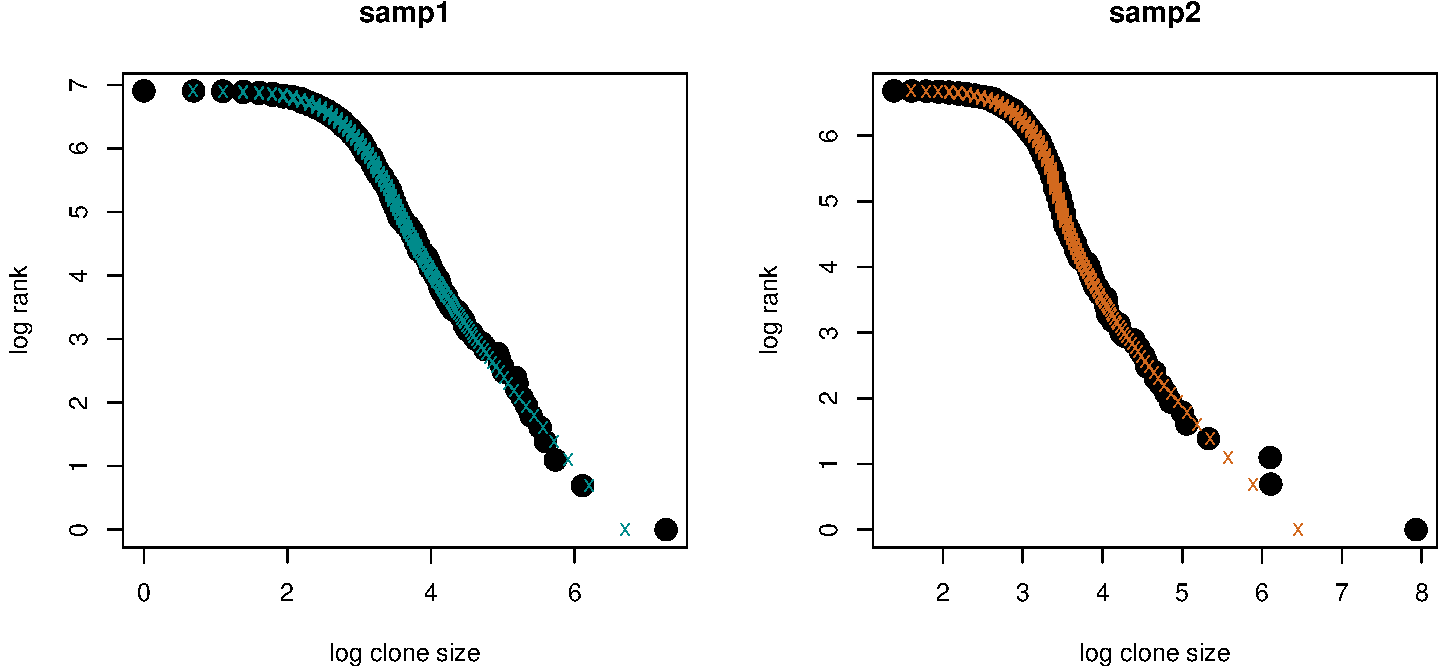
\includegraphics{powerTCR_files/figure-latex/unnamed-chunk-7-1} \end{adjustwidth}

The fits look pretty good!

Let's also try simulating data.

\begin{Shaded}
\begin{Highlighting}[]
\CommentTok{# Simulate 3 sampled repertoires}
\KeywordTok{set.seed}\NormalTok{(}\DecValTok{123}\NormalTok{)}
\NormalTok{s1 <-}\StringTok{ }\KeywordTok{rdiscgammagpd}\NormalTok{(}\DecValTok{1000}\NormalTok{, }\DataTypeTok{shape =} \DecValTok{3}\NormalTok{, }\DataTypeTok{rate =} \NormalTok{.}\DecValTok{15}\NormalTok{, }\DataTypeTok{u =} \DecValTok{25}\NormalTok{, }\DataTypeTok{sigma =} \DecValTok{15}\NormalTok{,}
                    \DataTypeTok{xi =} \NormalTok{.}\DecValTok{5}\NormalTok{, }\DataTypeTok{shift =} \DecValTok{1}\NormalTok{)}
\NormalTok{## Warning in if (p < 0 | p > 1) \{: the condition has length > 1 and only the}
\NormalTok{## first element will be used}
\NormalTok{s2 <-}\StringTok{ }\KeywordTok{rdiscgammagpd}\NormalTok{(}\DecValTok{1000}\NormalTok{, }\DataTypeTok{shape =} \FloatTok{3.1}\NormalTok{, }\DataTypeTok{rate =} \NormalTok{.}\DecValTok{14}\NormalTok{, }\DataTypeTok{u =} \DecValTok{26}\NormalTok{, }\DataTypeTok{sigma =} \DecValTok{15}\NormalTok{,}
                    \DataTypeTok{xi =} \NormalTok{.}\DecValTok{6}\NormalTok{, }\DataTypeTok{shift =} \DecValTok{1}\NormalTok{)}
\NormalTok{## Warning in if (p < 0 | p > 1) \{: the condition has length > 1 and only the}
\NormalTok{## first element will be used}
\NormalTok{s3 <-}\StringTok{ }\KeywordTok{rdiscgammagpd}\NormalTok{(}\DecValTok{1000}\NormalTok{, }\DataTypeTok{shape =} \DecValTok{10}\NormalTok{, }\DataTypeTok{rate =} \NormalTok{.}\DecValTok{3}\NormalTok{, }\DataTypeTok{u =} \DecValTok{45}\NormalTok{, }\DataTypeTok{sigma =} \DecValTok{20}\NormalTok{,}
                    \DataTypeTok{xi =} \NormalTok{.}\DecValTok{7}\NormalTok{, }\DataTypeTok{shift =} \DecValTok{1}\NormalTok{)}
\NormalTok{## Warning in if (p < 0 | p > 1) \{: the condition has length > 1 and only the}
\NormalTok{## first element will be used}
\end{Highlighting}
\end{Shaded}

\textbf{NB:} it is possible to simulate data according to a distribution
that is totally unrealistic. For example, what if you chose a very
light-tailed gamma distribution and a comparatively very high threshold,
but insisted (using) \(\phi\)) that data be observed above the
threshold? Here is what happens:

\begin{Shaded}
\begin{Highlighting}[]
\NormalTok{bad <-}\StringTok{ }\KeywordTok{rdiscgammagpd}\NormalTok{(}\DecValTok{1000}\NormalTok{, }\DataTypeTok{shape =} \DecValTok{1}\NormalTok{, }\DataTypeTok{rate =} \DecValTok{2}\NormalTok{, }\DataTypeTok{u =} \DecValTok{25}\NormalTok{, }\DataTypeTok{sigma =} \DecValTok{10}\NormalTok{,}
                     \DataTypeTok{xi =} \NormalTok{.}\DecValTok{5}\NormalTok{, }\DataTypeTok{shift =} \DecValTok{1}\NormalTok{, }\DataTypeTok{phi =} \NormalTok{.}\DecValTok{2}\NormalTok{)}
\NormalTok{## Warning in if (p < 0 | p > 1) \{: the condition has length > 1 and only the}
\NormalTok{## first element will be used}
\KeywordTok{plot}\NormalTok{(}\KeywordTok{log}\NormalTok{(}\KeywordTok{sort}\NormalTok{(bad, }\DataTypeTok{decreasing =} \OtherTok{TRUE}\NormalTok{)), }\KeywordTok{log} \NormalTok{(}\DecValTok{1}\NormalTok{:}\DecValTok{1000}\NormalTok{), }\DataTypeTok{pch =} \DecValTok{16}\NormalTok{,}
     \DataTypeTok{xlab =} \StringTok{"log clone size"}\NormalTok{, }\DataTypeTok{ylab =} \StringTok{"log rank"}\NormalTok{, }\DataTypeTok{main =} \StringTok{"bad simulation"}\NormalTok{)}
\end{Highlighting}
\end{Shaded}

\begin{adjustwidth}{\fltoffset}{0mm}
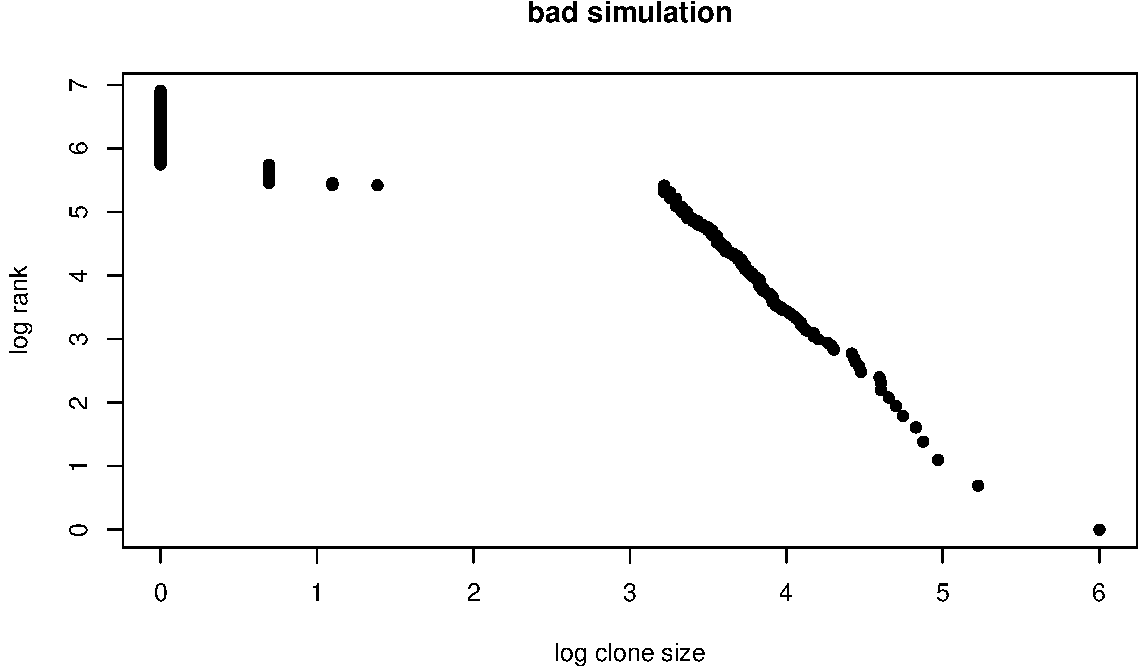
\includegraphics{powerTCR_files/figure-latex/unnamed-chunk-9-1} \end{adjustwidth}

Fun, but not too realistic for a clone size distribution. There are
several ways to go about finding reasonable parameters to simulate. One
intuitive and easy technique is to let real data speak for itself -- use
parameters similar to those obtained by fitting a distribution to true
TCR repertoire data sets.

\section{Doing comparative analysis}\label{doing-comparative-analysis}

Following the work in \textbf{my paper}, powerTCR provides the tools
needed to perform hierarchical clustering of TCR repertoire samples
according to their Jensen-Shannon divergence. We can test this out on
the 3 TCR repertoires we just simulated. First, we need to fit a model
to them. For computational efficiency, let's just supply the true
thresholds. Then, we can use \texttt{JS_spliced} to compute the
Jensen-Shannon divergence between each pair of theoretical distributions
corresponding to each of the TCR samples.

\texttt{JS_spliced} needs to be supplied the fitted model parameters as
well as a grid. The grid is important: it is the range over which each
distribution gets evaluated. If you are comparing a group of TCR
repertoires, the minimum value of your grid should be the smallest clone
size across all samples. The upper bound of the grid should be something
very large, say 100,000 or more. If you don't select a value large
enough, you will not be examining the tail of your fitted distributions
sufficiently, and the tail is important! The grid should also contain
every integer between its minimum and maximum. For computational
efficiency, here the upper bound on our grid is only 10,000.

\begin{Shaded}
\begin{Highlighting}[]
\CommentTok{# Fit model to the data at the true thresholds}
\NormalTok{sim_fits <-}\StringTok{ }\KeywordTok{list}\NormalTok{(}\StringTok{"fit1"} \NormalTok{=}\StringTok{ }\KeywordTok{fdiscgammagpd}\NormalTok{(s1, }\DataTypeTok{useq =} \DecValTok{25}\NormalTok{),}
                 \StringTok{"fit2"} \NormalTok{=}\StringTok{ }\KeywordTok{fdiscgammagpd}\NormalTok{(s2, }\DataTypeTok{useq =} \DecValTok{26}\NormalTok{),}
                 \StringTok{"fit3"} \NormalTok{=}\StringTok{ }\KeywordTok{fdiscgammagpd}\NormalTok{(s3, }\DataTypeTok{useq =} \DecValTok{45}\NormalTok{))}

\CommentTok{# Compute the pairwise JS distance between 3 fitted models}
\NormalTok{distances <-}\StringTok{ }\KeywordTok{matrix}\NormalTok{(}\KeywordTok{rep}\NormalTok{(}\DecValTok{0}\NormalTok{, }\KeywordTok{length}\NormalTok{(sim_fits)^}\DecValTok{2}\NormalTok{), }\DataTypeTok{nrow =} \KeywordTok{length}\NormalTok{(sim_fits))}
\KeywordTok{colnames}\NormalTok{(distances) <-}\StringTok{ }\KeywordTok{rownames}\NormalTok{(distances) <-}\StringTok{ }\KeywordTok{c}\NormalTok{(}\StringTok{"s1"}\NormalTok{,}\StringTok{"s2"}\NormalTok{,}\StringTok{"s3"}\NormalTok{)}

\NormalTok{grid <-}\StringTok{ }\KeywordTok{min}\NormalTok{(}\KeywordTok{c}\NormalTok{(s1,s2,s3)):}\DecValTok{10000}
\NormalTok{for(i in }\DecValTok{1}\NormalTok{:(}\KeywordTok{length}\NormalTok{(sim_fits)-}\DecValTok{1}\NormalTok{))\{}
    \NormalTok{for(j in (i}\DecValTok{+1}\NormalTok{):}\KeywordTok{length}\NormalTok{(sim_fits))\{}
        \NormalTok{distances[i,j] <-}\StringTok{ }\KeywordTok{JS_spliced}\NormalTok{(grid,}
                                     \DataTypeTok{shiftp =} \KeywordTok{min}\NormalTok{(sim_fits[[i]]$x),}
                                     \DataTypeTok{shiftq =} \KeywordTok{min}\NormalTok{(sim_fits[[j]]$x),}
                                     \DataTypeTok{phip =} \NormalTok{sim_fits[[i]]$mle[}\StringTok{'phi'}\NormalTok{],}
                                     \DataTypeTok{phiq =} \NormalTok{sim_fits[[j]]$mle[}\StringTok{'phi'}\NormalTok{],}
                                     \DataTypeTok{shapep =} \NormalTok{sim_fits[[i]]$mle[}\StringTok{'shape'}\NormalTok{],}
                                     \DataTypeTok{shapeq =} \NormalTok{sim_fits[[j]]$mle[}\StringTok{'shape'}\NormalTok{],}
                                     \DataTypeTok{ratep =} \NormalTok{sim_fits[[i]]$mle[}\StringTok{'rate'}\NormalTok{],}
                                     \DataTypeTok{rateq =} \NormalTok{sim_fits[[j]]$mle[}\StringTok{'rate'}\NormalTok{],}
                                     \DataTypeTok{threshp =} \NormalTok{sim_fits[[i]]$mle[}\StringTok{'thresh'}\NormalTok{],}
                                     \DataTypeTok{threshq =} \NormalTok{sim_fits[[j]]$mle[}\StringTok{'thresh'}\NormalTok{],}
                                     \DataTypeTok{sigmap =} \NormalTok{sim_fits[[i]]$mle[}\StringTok{'sigma'}\NormalTok{],}
                                     \DataTypeTok{sigmaq =} \NormalTok{sim_fits[[j]]$mle[}\StringTok{'sigma'}\NormalTok{],}
                                     \DataTypeTok{xip =} \NormalTok{sim_fits[[i]]$mle[}\StringTok{'xi'}\NormalTok{],}
                                     \DataTypeTok{xiq =} \NormalTok{sim_fits[[j]]$mle[}\StringTok{'xi'}\NormalTok{])}
    \NormalTok{\}}
\NormalTok{\}}

\CommentTok{# Distances are symmetric}
\NormalTok{distances <-}\StringTok{ }\NormalTok{distances +}\StringTok{ }\KeywordTok{t}\NormalTok{(distances)}
\end{Highlighting}
\end{Shaded}

Let's have a look at the distance matrix we just computed:

\begin{Shaded}
\begin{Highlighting}[]
\NormalTok{distances}
\NormalTok{##            s1         s2        s3}
\NormalTok{## s1 0.00000000 0.06839429 0.4488141}
\NormalTok{## s2 0.06839429 0.00000000 0.4101173}
\NormalTok{## s3 0.44881406 0.41011734 0.0000000}
\end{Highlighting}
\end{Shaded}

Note that, similarly, the function \texttt{JS_desponds} can be used to
compute the Jensen-Shannon divergence between samples if they were fit
using \texttt{fdesponds} rather than \texttt{fdiscgammagpd}.

We can use this distance matrix to perform hierarchical clustering. This
is done easily with the \texttt{clusterPlot} function.
\texttt{clusterPlot} is just a wrapper for \texttt{hclust}, and takes a
matrix of Jensen-Shannon distances like the one we just made, plus a
type of linkage. All possible types of linkage are listed in the help
file, but we recommend using complete linkage.

\begin{Shaded}
\begin{Highlighting}[]
\KeywordTok{clusterPlot}\NormalTok{(distances, }\DataTypeTok{method =} \StringTok{"complete"}\NormalTok{)}
\end{Highlighting}
\end{Shaded}

\begin{adjustwidth}{\fltoffset}{0mm}
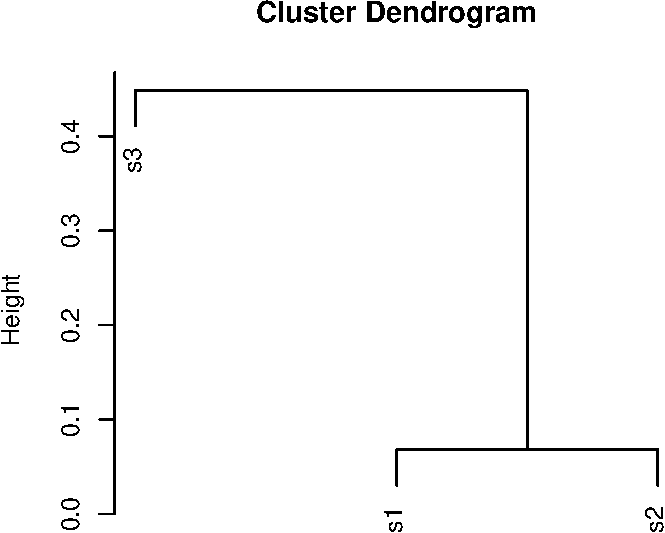
\includegraphics{powerTCR_files/figure-latex/unnamed-chunk-12-1} \end{adjustwidth}

The clustering result is exactly what we might expect. Indeed, we
simulated s1 and s2 using very similar parameter settings, so we should
expect them to be more closely related to each other than to s3. That is
exactly what the dendrogram displays.

\end{document}
